% Created 2023-10-16 lun 01:40
% Intended LaTeX compiler: pdflatex
\documentclass[11pt]{article}
\usepackage[utf8]{inputenc}
\usepackage[T1]{fontenc}
\usepackage{graphicx}
\usepackage{grffile}
\usepackage{longtable}
\usepackage{wrapfig}
\usepackage{rotating}
\usepackage[normalem]{ulem}
\usepackage{amsmath}
\usepackage{textcomp}
\usepackage{amssymb}
\usepackage{capt-of}
\usepackage{hyperref}
\usepackage{../modern}
\bibliography{fuentes.bib}
\raggedbottom
\setcounter{secnumdepth}{3}
\author{Luis Eduardo Galindo Amaya (1274895)}
\date{15 de Octubre del 2023}
\title{Interacción Humano Computadora}
\hypersetup{
 pdfauthor={Luis Eduardo Galindo Amaya (1274895)},
 pdftitle={Interacción Humano Computadora},
 pdfkeywords={},
 pdfsubject={},
 pdfcreator={Emacs 27.1 (Org mode 9.3)}, 
 pdflang={Spanish}}
\begin{document}

\modentitlepage{../images/escudo-uabc-2022-1-tinta-pos.png}
\tableofcontents
\pagebreak
\datasection{Individual}


\section{Introducción}
\label{sec:orgdc697f5}
La Interacción con los sistemas computaciones es indispensable para su 
utilizacion un buen diseño permite que el software tenga valor para los 
usuarios reduciendo la cantidad de aprendizaje y capacitacion necesaria para 
operarlo.


\section{Definicion}
\label{sec:orgb43d021}
\autocite{martinez_2007} La Interacción Humano-Computadora (HCI), es el 
estudio de la interacción entre el ser humano, las computadoras y las tareas 
que se desarrollan; principalmente se enfoca a conocer cómo la gente y las
computadoras pueden interactuar para llevar a cabo tareas por medio de sistemas
y software.

\pagebreak

\section{Modelo de diseño de la interaccion}
\label{sec:org940c38c}
el Modelo de diseño de la interaccion (MODIHC) permite diseñar todos los 
aspectos involucrados en la interacción entre un humano y una computadora 
cuando se están desarrollando productos de software \autocite{martinez_2007}. 

\begin{figure}[htbp]
\centering
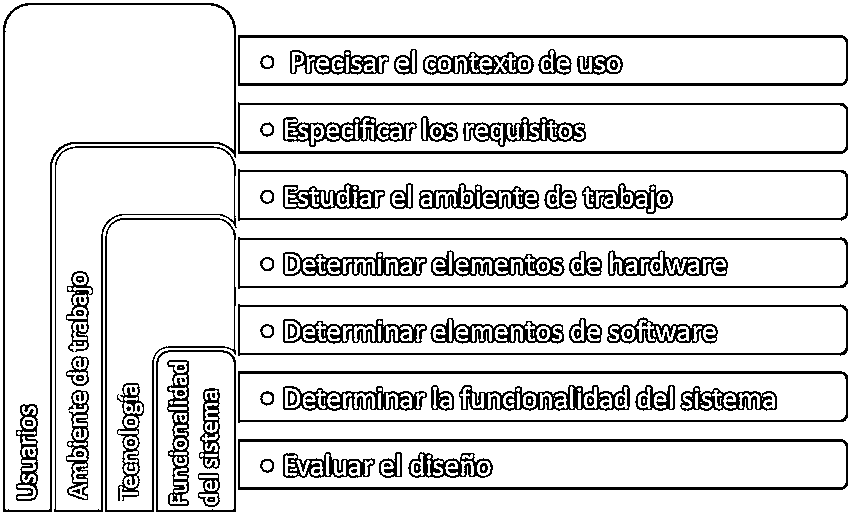
\includegraphics[width=9cm]{img/Design.png}
\caption{Componenter de MODIHC}
\end{figure}

\subsection{Componente usuarios}
\label{sec:orge1e9f82}
\autocite{narciso_valero_2008} Para la IHC, entender el aspecto físico, 
intelectual y la personalidad de los diferentes usuarios es un factor 
fundamental. Conocer quiénes y cómo usarán el producto de software permitirá 
generar un diseño que posteriormente se traducirá en un sistema en operación 
eficiente y usable. 

\subsection{Objetivos del componente usuario}
\label{sec:org314102f}
\autocite{narciso_valero_2008} Los objetivos que el diseñador de software 
debe alcanzar en este componente son los siguientes: 

\begin{itemize}
\item Identificar a todos los usuarios del producto de software.
\item Clasificar a los usuarios según sus características.
\item Conocer para qué y bajo qué condiciones se usará el producto de software.
\item Crear el perfil de usuarios. Determinar características de la IU basadas en los usuarios. Crear el documento de especificación de requisitos.
\end{itemize}


\subsection{Componente ambiente de trabajo}
\label{sec:org1551d75}
\autocite{narciso_valero_2008} Para el diseño de la IHC, es necesario 
realizar un estudio del ambiente en el cual va a operar el sistema 
computarizado y para ello hay que tomar en cuenta tres aspectos: el 
organizacional, el físico y el social. 

\subsection{Objetivos del componente de ambiente de trabajo}
\label{sec:org080f1fd}
\autocite{narciso_valero_2008} Los objetivos que el diseñador de software
debe alcanzar en este componente son los siguientes: 

\begin{itemize}
\item Estudiar los aspectos organizacionales, físicos y sociales del ambiente de trabajo.
\item Conocer la distribución del espacio físico y del trabajo.
\item Localizar equipos y materiales de oficina.
\item Crear el \textbf{documento de especificación del ambiente de trabajo}.
\item Determinar características de la IU basadas en el ambiente de trabajo.
\end{itemize}

\subsection{Componente Funcionalidad del Sistema}
\label{sec:org7f64201}
\autocite{narciso_valero_2008} El diseñador de software debe estudiar el 
modelo mental que cada uno de los usuarios tiene sobre el sistema y cómo 
razonan con respecto a sus funciones. Luego, debe ―mezclar‖ estos diferentes 
modelos mentales para así determinar, mediante la IU, la funcionalidad correcta 
del sistema. Además, debe conocer las preferencias de los usuarios para 
determinar lo que ellos encontrarán aceptable como un sistema usable.

\subsection{Objetivos del componente funcionalidad del sistema}
\label{sec:org0351ac2}
\autocite{narciso_valero_2008} Los objetivos que el diseñador de software
debe alcanzar en este componente son los siguientes: 

\begin{itemize}
\item Identificar las necesidades de la organización que debe satisfacer el producto de software.
\item Identificar las metas y requisitos de los usuarios que deben cumplirse mediante el uso del producto de software.
\item Estudiar el modelo mental que cada usuario tiene del sistema.
\item Estudiar las características de la IU definidas en los componentes anteriores.
\item Estudiar la información obtenida de la fase de análisis del método o metodología de desarrollo de software que se aplique.
\item Diseñar una IU que represente de manera apropiada la funcionalidad del sistema.
\end{itemize}


\subsection{Componente Tecnología}
\label{sec:orgcfc11d5}
\autocite{narciso_valero_2008} Para diseñar la IHC, desde el punto de 
vista de la tecnología, es necesario determinar en primer lugar los 
dispositivos de entrada/salida apropiados para la interacción con dicho 
sistema, tomando en cuenta la disponibilidad o posibilidad de adquisición de 
los mismos dentro de la organización, y en segundo lugar los diferentes estilos
de interacción (elementos de software), teniendo siempre en mente a los 
usuarios, la funcionalidad del sistema y el ambiente de trabajo. 

\subsection{Objetivos del componente componente tecnología}
\label{sec:org65bee05}
\autocite{narciso_valero_2008} Los objetivos que el diseñador de software
debe alcanzar en este componente son los siguientes:

\begin{itemize}
\item Seleccionar los dispositivos de entrada/salida que mejor se adapten al usuario, al ambiente de trabajo y a la disponibilidad de recursos de la organización.
\item Seleccionar los estilos de interacción apropiados para el producto de software a desarrollar.
\item Determinar características de la IU basadas en la Tecnología.
\end{itemize}


\section{Conclusión}
\label{sec:org7d0bb94}
Durante este taller investigue sobre como diseñar las interacciones entre los 
usuarios y las computadoras, esto fue bastante interesante porque pensaba que 
que al referirse a 'interacciona' solamente se refreía a los periférico de la 
computadora, ahora entiendo que el diseño de interacciones se refiere a diseñar 
software que los usuarios puedan entender.  

\section{Referencias}
\label{sec:orgd95483e}
\printbibliography[heading=none]
\end{document}
